
\documentclass[11pt]{article}
% 11 point fonts

\usepackage{graphicx}
\usepackage{fixltx2e}
% for importing images

\usepackage[top = 1 in, bottom = 1 in, left = 0.5 in, right = 0.5 in]{geometry}
%margins

\begin{document}

\title{Physics Behind the Simulation:\\
	A CS296 Report by Group 18.}
	
\author{Rohit Kumar \\
		\textup{Roll No 120050028} \\
		\textit{rohit@cse.iitb.ac.in}
	\and
	Suman Sourabh \\
	\textup{Roll No 120050031} \\
	\textit{sumansourabh26@cse.iitb.ac.in}
	\and
	Nitin Chandrol\\
	\textup{Roll No 120050035} \\
	\textit{ntnchandrol@cse.iitb.ac.in}
	}

\date{\today}

\maketitle

\section{Introduction}

	\paragraph{}
	The purpose of this report is to explain the simulation of the three new Box-2D\cite{box} blocks added to the system. It attemps to explain 
	the motion of the Box2D elements using the laws of physics and the mathematical equations governing them. Through this report, our team also
	aim to learn basic Latex commands\cite{andyroberts}. 
 
 
\section{Physics behind the simulation}
\paragraph{}
These 3 subsections explains in detail, the Box2D blocks using laws and equations of physics:
	The three new elements that we have added are:
	
	\begin{enumerate}
	\item Hinged rod with wedge, dominoes and sphere
	\item bet
	\item gam
	\end{enumerate}

\subsection{Hinged rod with wedge, dominoes and sphere}
\paragraph{}

	This section is governed by the laws of conservation of energy, momentum and angular momentum.
	The potential energy of the falling sphere is converted into kinetic energy which appears in the 
	velocity of sphere. Upon collision it's energy is transferred to rod with conservation of angular momentum
	(as no external torque is applied).
	Further the rod collides with the wedge which further collides with dominoes.
	The energy conservation is governed by the equation:
	
	\begin{equation}
		U_1 - U_2 = \frac{1}{2}m \vec{v}.\vec{v}
	\end{equation}

Here, 	
\begin{itemize}
\item U\textsubscript{1} is the initial potential energy of the sphere
\item U\textsubscript{2} is the potential energy of the sphere at the time of collision with hinged rod
\item m is the mass of the sphere
\item v is the velocity of the sphere at the time of collision
\end{itemize}

	
\begin{center}
  \includegraphics[scale = 0.4]{ob1} \\
  \emph{A screenshot of this block} \\
\end{center}

\paragraph{}
In collision of sphere with hinge, the net external torque is zero. So, angular momentum is conserved.

\begin{equation}
		\Gamma =  \frac{\mathrm{d} \vec{L}}{\mathrm{d} t}
\end{equation}

Here, 	
\begin{itemize}
\item L is the net angular momentum of the system of rod and sphere about the hinge
\item I is the net external torque
\item t is time
\end{itemize}


\subsection{Box2D top level block 2}

This section describes the collision of two spheres. The momentum is conserved according to the following equation:

\begin{equation}
		\Gamma =  \frac{\mathrm{d} \vec{L}}{\mathrm{d} t}
\end{equation}

Here, 	
\begin{itemize}
\item m\textsubscript{1} is the mass of first sphere
\item m\textsubscript{2} is the mass of second sphere
\item v\textsubscript{2} is the velocity of second sphere
\item v\textsubscript{2} is the velocity of second sphere
\end{itemize}

\begin{center}
  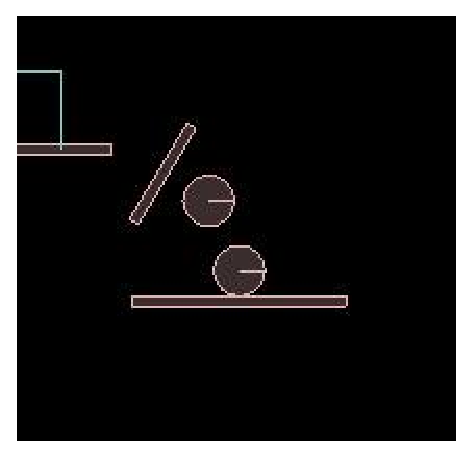
\includegraphics[scale = 1]{ob2} \\
  \emph{A screenshot of this block} \\
\end{center}



\subsection{Box2D top level block 3}

\begin{center}
  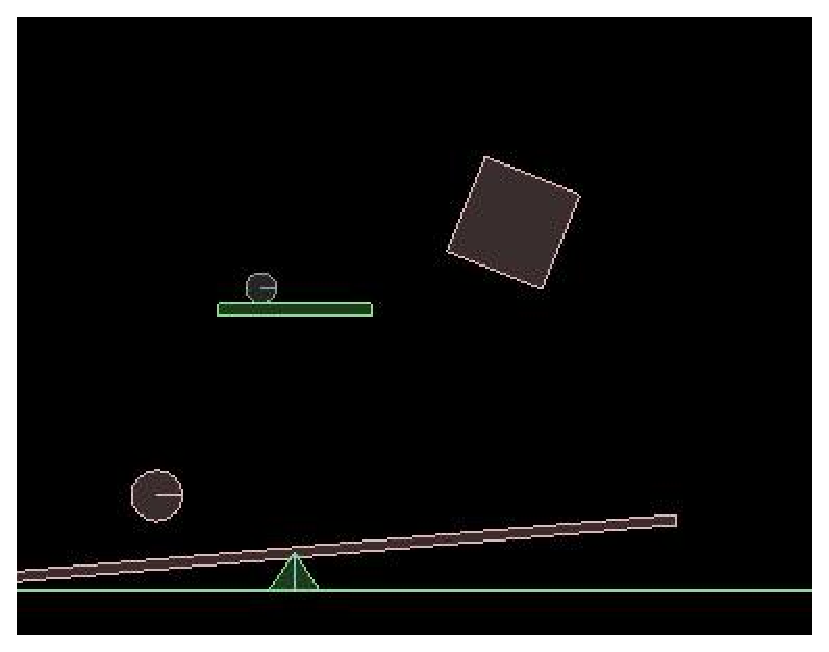
\includegraphics[scale = 1]{ob3} \\
  \emph{A screenshot of this block} \\
\end{center}

Square box undergoes a projectile motion after leaving the see-saw plank and finally collides with the ball placed on upper plank.
The projectile motion is described as:

\begin{equation}
	\vec{v_1} = \vec{u_1} - \vec{g}t
\end{equation}
\section{Conclusions}
	We conclude the document.

\bibliographystyle{plain}
\bibliography{biblo}

\end{document}


